\section{Results}

At the outset of the test, after an explanation of what the product was intended to allow a person to achieve, the interface was shown to the participant and they were asked to give their initial impressions.  \\
One of the first things they noted about the application was the lack of what they felt was a "standard" layout.  More specifically, they commented on how there was no main menu present at the top of the window but instead large labelled action buttons arranged around the primary canvas area.  However, they also said that they thought it looked pretty straight forward to use by appearance alone.

The first test was to load an image file that had been placed on the user's desktop.  This took 56 seconds to complete but only five clicks of the mouse.  The operation took a relatively long time because some considerable searching was required by the user to find the relevant button.  This confusion was attributed by them to the lack of a File menu with an Open item which they feel is fairly standard in most applications they use.  The participant scored it a 3 out of 5 for usability and said that it was easy enough to do, they just couldn't find the right user interface control to start the operation.

The second and third tests were to add an annotation followed by a second annotation.  On both occasions the participant successfully created them in around five seconds with slight variances in the number of clicks required relating directly to the size of the polygon they drew.  They found this extremely simple and gave this feature a usability rating of one - meaning easy.

The fourth task they were set was to select a previously created annotation and this took 43 seconds to complete with five clicks required.  Initially there was some confusion during this test because the user tried to click on the edge of the polygon to select it.  When this did not work, and they ended up creating another polygon by mistake, they hunted around looking at the interface more closely.  Eventually they discovered the labels of the annotations on the far right of the window and completed the selection.  The participant stated that they would have preferred if the list of annotations were placed in a more prominent position and gave this feature a 3 out of 5.

The fifth task was to delete an annotation that they had made.  This took 6 seconds to complete with only one click.  The user said that they were happy that this was an easy operation giving it a score of one.

The sixth test was to edit an annotation.  The user was prompted to increase the size of their polygon and then to change its name.  These actions took 8 and 15 seconds respectively with a click required for each.  The participant stated that again this was an easy operation to complete but that they wished the list of annotations were nearer the canvas area.  They gave this a score of 2

Duplicating an annotation was the seventh task and was completed in two clicks over a period of four seconds.  This was considered easy by the test's participant and they gave this a score of 1.

The final task asked of the user was to save the annotated image to a file.  This took seven seconds, two clicks, and they stated it was extremely easy, again giving this a score of one.  This experiment was then repeated for a second image and then again for the first image.  All measurements recorded for these subsequent operations can be seen in Appendix \ref{Appendix}.

In conclusion, The analysis given above can be summarized in Figure \ref{fig:plot}. Line segments with large slops indicate that user performance has change dramatically from one experiment to the other.

\begin{figure}[t]
\centering
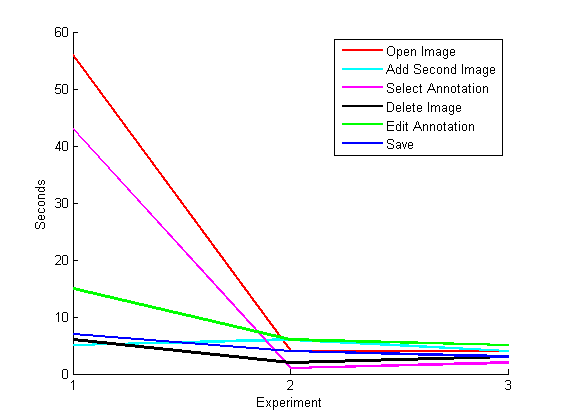
\includegraphics[width=8cm]{obs_sec.png}
\caption{Plot of user performance in 3 experiments. User had some difficulties initially in opening an image and selecting an annotation}
\label{fig:plot}
\end{figure}
